\documentclass[xcolor=dvipsnames]{beamer} 
\useoutertheme{infolines} 
\usetheme{CambridgeUS} 
%\setbeamertemplate{items}[ball] 
\setbeamertemplate{blocks}[rounded][shadow=true] 
\setbeamertemplate{navigation symbols}{} 
\setbeamercolor{block title}{fg=darkred}
\setbeamercolor{local structure}{fg=darkred}
\usepackage[ngerman]{babel}
\usepackage[latin1]{inputenc}
\usepackage{wrapfig}
\usepackage{subcaption}
\addtobeamertemplate{block begin}{\setlength{\textwidth}{0.9\textwidth}}{}

\usepackage[style=numeric, sorting=none]{biblatex} 
\usepackage[justification=raggedright,compatibility=false,singlelinecheck=false,labelfont=bf]{caption}
\addbibresource{citations.bib}%the bibliography database 
\DeclareFieldFormat{journaltitle}{#1}         
%\DeclareFieldFormat{month}{}           
\DeclareFieldFormat[article]{title}{}
\DeclareFieldFormat[article]{volume}{\mkbibbold{#1}\addcomma\space} 
\DeclareFieldFormat[article]{number}{\space #1}
\DeclareFieldFormat{url}{} 
\DeclareFieldFormat{doi}{}
\DeclareFieldFormat{pages}{}
\renewcommand*{\multinamedelim}{\addcomma\space}
\renewcommand*{\finalnamedelim}{\addcomma\space} 
\renewcommand*{\labelnamepunct}{\addcomma\space}
\renewcommand*{\bibpagespunct}{\adddot\space}
\renewbibmacro{in:}{}

\title[Synchronisation in Netzwerken\hspace{12mm} \insertframenumber/
\inserttotalframenumber]{Synchronisation in Netzwerken:\\Master Stability Function und
Permutationssymmetrien}
\institute[]{Institut fur Theoretische Physik, Technische Universitat Berlin, Germany}



\author[F. Zimmermann, H. Taher, P. Affeld]{
	\underline{Felix Zimmermann, Halgurd Taher, Paul-Rainer Affeld}
}

\date[\today]{\today}

\renewcommand{\familydefault}{times}
\renewcommand{\rmdefault}{times}
\setcounter{MaxMatrixCols}{20}


\begin{document}


\frame{
	\titlepage
	\begin{figure}
		\includegraphics[width=0.12\textwidth]{abb/tulogo.pdf}
	\end{figure}
}


\frame{
	\frametitle{Inhalt}
	\tableofcontents
}

\section{Einleitung}
\frame{

	\frametitle{Einleitung}
	\tableofcontents[currentsection]

}

\frame{
	\frametitle{Dynamik auf Netzwerken}
		\begin{itemize}
		\item $N$ miteinander gekoppelte Knoten
		\item Jeder Knoten wird durch dynamische Gleichung beschrieben
	
	\begin{align}\label{eq:dyneqcommon}
					\overset{\cdot}{\boldsymbol{x}}_i(t)&=\boldsymbol{f}(\boldsymbol{x}_i(t))+\sigma\sum_j A_{ij}\boldsymbol{h}(\boldsymbol{x}_j)
					\\\notag & i=1,...,N
					\\\notag & A_{ij}\text{ Kopplungsmatrix}
					\\\notag & \boldsymbol{f},\boldsymbol{h}:\mathbb{R}^n\rightarrow\mathbb{R}^n
	\end{align}
	\item
	Definiere
	\begin{align*}
	\boldsymbol{X}=\left(\boldsymbol{x}_1,...,\boldsymbol{x}_N\right)^{\text{T}},
	\boldsymbol{F}=\left(\boldsymbol{f}(\boldsymbol{x}_1),...,\boldsymbol{f}(\boldsymbol{x}_N)\right)^{\text{T}},
	\boldsymbol{H}=\left(\boldsymbol{h}(\boldsymbol{x}_1),...,\boldsymbol{h}(\boldsymbol{x}_N)\right)^{\text{T}}
	\end{align*}
	$\Rightarrow$ �quivalente Gleichung zu (1) 
	\begin{align*}
	\overset{\cdot}{\boldsymbol{X}}(t)=\boldsymbol{F}(\boldsymbol{X}(t))+\sigma\boldsymbol{A}\otimes\boldsymbol{H}(\boldsymbol{X}(t))
	\end{align*}
		\end{itemize}
}

\section{Synchronisation I}
\frame{
	\frametitle{Synchronisation I}
	\tableofcontents[currentsection]

}

\frame{
	\frametitle{Synchronisation I}
	Globale Synchronisation liegt vor wenn 
	\begin{align*}
		\boldsymbol{x}_1(t)=\boldsymbol{x}_2(t)=...=\boldsymbol{x}_N(t)=:\boldsymbol{s}(t)
	\end{align*}
	erf�llt ist.\\
	$ $\\
	Stabilit�t der Synchronisation :\\
	Wie entwickelt sich kleine Abweichung von $\boldsymbol{s}(t)$ zeitlich weiter?
	\begin{itemize}
\item
	Linearisierung um $\boldsymbol{s}(t)$ $\Rightarrow$	Master Stability Equation (MSE) :
	\begin{align*}
			\delta\overset{\cdot}{\boldsymbol{X}}(t)=
			\left[D\boldsymbol{F}(\boldsymbol{s}(t))+\sigma\boldsymbol{A}\otimes D\boldsymbol{H}(\boldsymbol{s}(t))\right]\delta\boldsymbol{X}(t)
	\end{align*}
	\end{itemize}
}

\frame{
	\frametitle{Master Stability Function}
	Ljapunow-Exponenten $\lambda_i$
		\begin{align*}
		\lambda_i=\lim_{t\rightarrow\infty}\frac{1}{t} ln\left(\frac{|\delta \boldsymbol{x}_i(t)|}{|\delta \boldsymbol{x}_i(0)|}\right)
		\end{align*}
	Master Stability Function (MSF) $\Lambda$ ist gr��ter Ljapunow Exponent
	\begin{itemize}
	\item $\Lambda>0$, Synchronisation instabil, Fehler w�chst, Bahnkurven $\boldsymbol{x}_i$(t) entfernen sich von $\boldsymbol{s}$(t)
	\item $\Lambda<0$, Synchronisation stabil, Fehler schrumpft, Bahnkurven $\boldsymbol{x}_i$(t) n�hern sich wieder $\boldsymbol{s}$(t)
	\end{itemize}
}

\frame[t]{
	\frametitle{Voraussetzungen f�r Synchronisation}
   	\begin{itemize}
   	\item jeder Knoten ben�tigt gleichen Input
   	\item setzt u.a. konstante Zeilensumme von $\boldsymbol{A}$ voraus
   	\end{itemize}
}

\frame{
	\frametitle{Voraussetzungen f�r Synchronisation}
   	\begin{itemize}
   	\item jeder Knoten ben�tigt gleichen Input
   	\item setzt u.a. konstante Zeilensumme von $\boldsymbol{A}$ voraus
   	\end{itemize}
   	Im Allgemeinen nicht erf�llt, z.B. :
    \begin{align*}
    \boldsymbol{A}_1=
        \begin{pmatrix}
                   0 & 1 & 1 & 1 & 0 & 1 & 1 & 1 & 1 & 1 & 1 \\
                   1 & 0 & 1 & 1 & 1 & 1 & 0 & 1 & 1 & 1 & 1 \\
                   1 & 1 & 0 & 1 & 1 & 1 & 1 & 1 & 0 & 1 & 1 \\
                   1 & 1 & 1 & 0 & 1 & 1 & 1 & 1 & 1 & 1 & 1 \\
                   0 & 1 & 1 & 1 & 0 & 1 & 1 & 1 & 1 & 1 & 0 \\
                   1 & 1 & 1 & 1 & 1 & 0 & 1 & 1 & 1 & 1 & 1 \\
                   1 & 0 & 1 & 1 & 1 & 1 & 0 & 1 & 1 & 1 & 1 \\
                   1 & 1 & 1 & 1 & 1 & 1 & 1 & 0 & 1 & 0 & 1 \\
                   1 & 1 & 0 & 1 & 1 & 1 & 1 & 1 & 0 & 1 & 1 \\
                   1 & 1 & 1 & 1 & 1 & 1 & 1 & 0 & 1 & 0 & 0 \\
                   1 & 1 & 1 & 1 & 0 & 1 & 1 & 1 & 1 & 0 & 0 
        \end{pmatrix}
    \end{align*}
   	Zeilensumme NICHT konstant
   
}
\section{Simulationsbeispiel}
\frame{
	\frametitle{Simulationsbeispiel}
	\tableofcontents[currentsection]

}
\frame{
	\frametitle{Beispiel}
	\begin{itemize}
	\item Diskretes System mit $N=11$ Knoten
	\item Kopplungsmatrix $\boldsymbol{A}_1$
	\item Diskrete dynamische Gleichung gegeben durch
	\begin{align*}
	x_i^{t+1}&=\left[\beta\mathcal{I}(x_i^t)+\sigma \sum_j^N A_{ij}\mathcal{I}(x_j^t)+\delta\right] \text{mod}\quad 2\pi
	\\\notag & \beta,\sigma \text{ Kopplungsparameter}
	\\\notag &\mathcal{I}(x)=\frac{1-Cos(x)}{2}
	\end{align*}
	\end{itemize}

	(aus Pecora et. al 2014)
}

\frame{
	\frametitle{Beispiel}
	\centering
	%\href{run:C:/Users/Halgurd/Documents/_TUBerlin/Kontrolle und Dynamik 2015/ProjectMSF/ClusterNum/ClusterNum/bin/Release/ClusterNum.exe}
	%{Simulation des Beispiels}
	Simulation des Beispiels
   
}
\frame{
	\frametitle{Beobachtungen}
	\begin{itemize}
		\item Keine globale Synchronisation
		\item  5 Gruppen von Knoten die sich synchron verhalten
		\item $\Rightarrow$ Cluster
	\end{itemize}
	\begin{figure}
		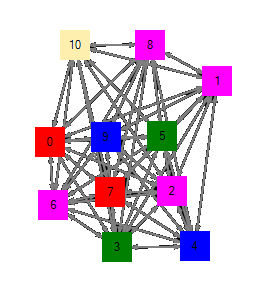
\includegraphics[width=0.75\textwidth]{abb/cluster.png}
	\end{figure}
}

\section{Cluster und Permutationssymmetrien}
\frame{
	\frametitle{Cluster und Permutationssymmetrien}
	\tableofcontents[currentsection]

}
\frame{
	\frametitle{Cluster}
	$\boldsymbol{A}_1$ hat zwar global keine konstante Zeilensumme aber:
	\begin{itemize}
	\item Forderung nach gleichem Input f�r jeden Knoten kann \underline{innerhalb} eines Cluster erf�llt werden\\
	   (da gleiche Zeilensumme innerhalb eines Clusters f�r z.b. $\boldsymbol{A}_1$)
	\item Knoten k�nnen vertauscht werden ohne Dynamik zu �ndern
	\end{itemize}
	$\Rightarrow$ Netzwerk besitzt offensichtlich Symmetrien\\
	Suche nach Permutationssymmetrien sinnvoll:
	\begin{itemize}
	\item mathematisch beschrieben durch Permutationsmatrizen $\boldsymbol{P}_i$
	\item $\boldsymbol{A}=\boldsymbol{P}\boldsymbol{A}\boldsymbol{P}^{-1} \Rightarrow \boldsymbol{A}$ bleibt unver�ndert bei Tauschen der Knoten
	\end{itemize}
   
}
\frame{
	\frametitle{Permutationssymmetrien}
	Beispiele f�r Permutationssymmetrien:
	\begin{itemize}
	\item Knoten 1 und 2 vertauschbar \\$\Rightarrow$ 
			1 und 2 im Cluster
	\item Knoten 1 und 2 nur vertauschbar\\ 
	bei gleichzeitiger Vertauschung von 3 und 4\\$\Rightarrow$ 
			Cluster (1,2) und (3,4) "verschr�nkt" (Pecora et al.: interwinded)
	\end{itemize}
}
\frame{
	\frametitle{Cluster}
	\begin{itemize}
	\item Clustersuche in der Regel numerisch
	\item Bibliothek nauty liefert $M$ Cluster 	\begin{tiny}\href{http://pallini.di.uniroma1.it/}{http://pallini.di.uniroma1.it/}	\end{tiny}
	\item Nach Finden der Cluster kann St�rung umgeschrieben werden:
	\end{itemize}
	\begin{align*}
		\delta\overset{\cdot}{\boldsymbol{X}}(t)&=	
		\left[D\boldsymbol{F}(\boldsymbol{s}(t))+\sigma\boldsymbol{A}\otimes D\boldsymbol{H}(\boldsymbol{s}(t))\right]\delta\boldsymbol{X}(t)\\&=
				\left[\sum_{m=1}^{M} \boldsymbol{E}^{(m)} \otimes D\boldsymbol{F}(\boldsymbol{s}_m(t))+\sigma\boldsymbol{A}\otimes \boldsymbol{I}_n\sum_{m=1}^{M} \boldsymbol{E}^{(m)}\otimes D\boldsymbol{H}(\boldsymbol{s}_m(t))\right]\boldsymbol{X}(t)
		\\\notag & \boldsymbol{s}_m(t) \text{ ist synchroner Orbit des Clusters }m
		\\\notag & \boldsymbol{E}^{(m)}_{ii} =1\text{ wenn Knoten }i\text{ zum Cluster }m\text{ geh�rt}
	\end{align*}
	\hspace{10pt}

}
\section{Synchronisation II}
\frame{
	\frametitle{Synchronisation II}
	\tableofcontents[currentsection]

}
\frame{
	\frametitle{Formen von Synchronisation}
	\begin{itemize}
	\item globale Synchronisation\\
	alle Knoten des Netzwerks synchron
	\item isolierte Synchronisation innerhalb eines Clusters\\
	alle Knoten eines Clusters synchron
	\item gemeinsame Synchronisation zweier Cluster\\
		 zwei Cluster zeigen gleichzeitig isolierte Synchronisation
	\end{itemize}

}
\frame{
	\frametitle{Isolierte Synchronisation}
	Warum kann ein Cluster synchron sein w�hrend andere nicht synchron sind?
	\begin{itemize}
	\item
		Betrachte Dynamik eines Knotens aus Cluster A unter Permutation von Cluster B (A wird nicht ver�ndert):
	\begin{figure}
		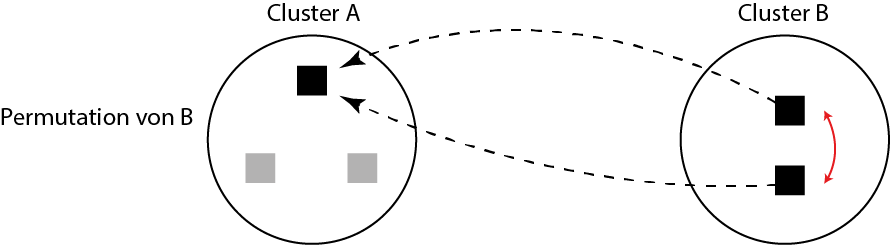
\includegraphics[width=0.75\textwidth]{abb/perm_b.png}
	\end{figure}
	\item 
		Da sich bei Permutationssymmetrie die Dynamik nicht �ndert, muss jeder Knoten aus B gleich starken Input an einen Knoten aus A geben.
\end{itemize}
}

\frame{
	\frametitle{Isolierte Synchronisation}
	Warum kann ein Cluster synchron sein w�hrend andere nicht synchron sind?
	\begin{itemize}
	\item
		Betrachte nun Dynamik eines Knotens aus Cluster A unter Permutation dieses Clusters	(B wird nicht ver�ndert):
	\begin{figure}
		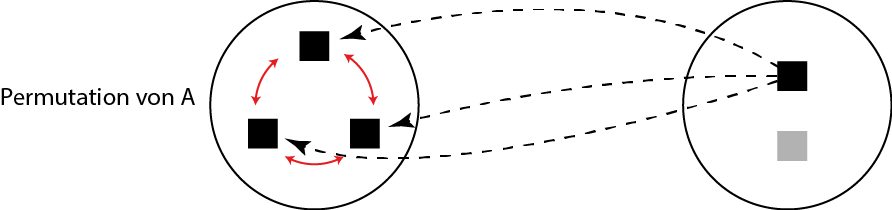
\includegraphics[width=0.75\textwidth]{abb/perm_a.png}
	\end{figure}
	\item
		Auch hier: Dynamik bleibt gleich. 
	\item 
		Folglich ist ein Knoten aus B ist gleich an jeden Knoten aus A gekoppelt.
\end{itemize}
}

\frame{
	\frametitle{Isolierte Synchronisation}
	Warum kann ein Cluster synchron sein w�hrend andere nicht synchron sind?
	\begin{itemize}
	\item		
		Zusammen: Jeder Knoten in B bekommt in der Summe den gleichen Input vom Cluster A, egal ob dieser synchron oder nicht ist.
	\\
	$\Rightarrow$ Wenn Permutationsmatrizen existieren, die die Cluster getrennt permutieren, existiert isolierte Synchronisation
	\item
	 Isolierte Synchronisation \underline{nicht} bei "verschr�nkten" Clustern\\
			(Permutation ver�ndert beide Cluster)
\end{itemize}
}
\section{Lokale Stabilit�tsanalyse}
\frame{
	\frametitle{Lokale Stabilit�tsanalyse}
	\tableofcontents[currentsection]

}
\frame{
	\frametitle{Stabilt�t der Clustersynchronit�t}
	Stabilit�tsanalyse:
	\begin{itemize}
	\item f�r einzelne Cluster schwierig:\\in welche Richtung sollte $\delta\boldsymbol{X}$ betrachtet werden?
	\item $\Rightarrow$ Basistransformation mit Transformationsmatrix $\boldsymbol{T}$
	\item $\boldsymbol{T}$ blockdiagonalisiert $\boldsymbol{A}$
	\item oberer $M$x$M$ Block beschreibt die Bewegung innerhalb der Synchronisationsmannigfaltigkeit 
	\end{itemize}
	\begin{figure}
			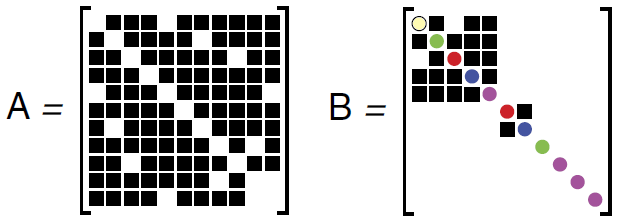
\includegraphics[width=0.6\textwidth]{abb/ABMat.png}
	\end{figure}
	(Pecora et al. 2014)
}

\frame{
	\frametitle{MSF f�r Cluster}
	Nach Transformation durch $\boldsymbol{T}$ ergibt sich linearisierte St�rung $\boldsymbol{\eta}$ in neuer Basis
		\begin{align*}
		\overset{\cdot}{\boldsymbol{\eta}}(t)&=
				\left[\sum_{m=1}^{M} \boldsymbol{J}^{(m)} \otimes D\boldsymbol{F}(\boldsymbol{s}_m(t))+\sigma\boldsymbol{B}\otimes \boldsymbol{I}_n\sum_{m=1}^{M} \boldsymbol{J}^{(m)}\otimes D\boldsymbol{H}(\boldsymbol{s}_m(t))\right]\boldsymbol{\eta}(t)
		\\\notag &\boldsymbol{\eta}(t)=\boldsymbol{T}\otimes\boldsymbol{I}_n\delta\boldsymbol{X}(t)
		\\\notag & \boldsymbol{B}=\boldsymbol{T}\boldsymbol{A}\boldsymbol{T}^{-1}
		\\\notag & \boldsymbol{J}^{(m)}=\boldsymbol{T}\boldsymbol{E}^{(m)}\boldsymbol{T}^{-1}
		\end{align*}
		aus dieser MSE kann MSF f�r jedes Cluster (lokal) berechnet werden
}

\frame{
	\frametitle{Simulation lokale MSF}
	\centering
	Stabilit�tsanalyse
}
\frame{
	\frametitle{Simulation lokale MSF}
	\centering
		\begin{figure}
			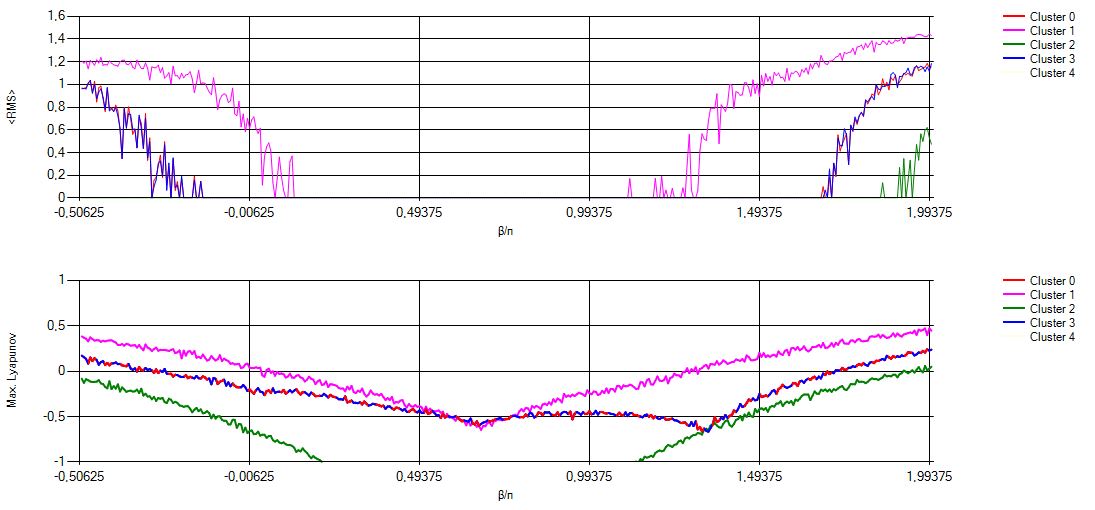
\includegraphics[width=1\textwidth]{abb/ljapunow.png}
		\end{figure}
}
\section{Fazit}
\frame{
	\frametitle{Fazit}
	\tableofcontents[currentsection]

}
\frame{
	\frametitle{Fazit}
	\begin{itemize}
	\item globale Stabilit�tsanalyse �ber MSF setzt konstante Zeilensumme voraus
	\item In Netzwerken mit Symmetrien existieren Cluster
	\item Knoten eines Cluster k�nnen synchron laufen

	\item lokale Stabilit�tsanalyse der Synchronisation durch Basistransformation m�glich
	\item Isolierte Desynchronisation bei nicht verschr�nkten (non intertwined) Clustern m�glich
	\end{itemize}
}

\end{document}